\twocolumn
\subsubsection{ Implementación con un tiempo de muestreo de 10 veces el ancho de banda del sistema
}


Si muestreamos 10 veces el ancho de banda:
\[
f_s = 10 f_{\mathrm{bw}}, \qquad T = \frac{1}{f_s}.
\]

La simulación se realiza con:
\[
\texttt{sim\_pid\_euler\_ideal(G,\,T,\,Kp,\,Ti,\,Td,\,1);}
\]

En la Figura~\ref{fig:fs10} se observa que la respuesta discreta no reproduce bien a la continua: se introduce más retardo y el seguimiento al escalón empeora.
Un muestreo de 10 veces el ancho de banda apenas alcanza para representar la dinámica dominante. El efecto combinado del ZOH y la discretización generan un retardo en la fase, reduciendo el desempeño.  

\begin{figure}[!t]
	\centering
	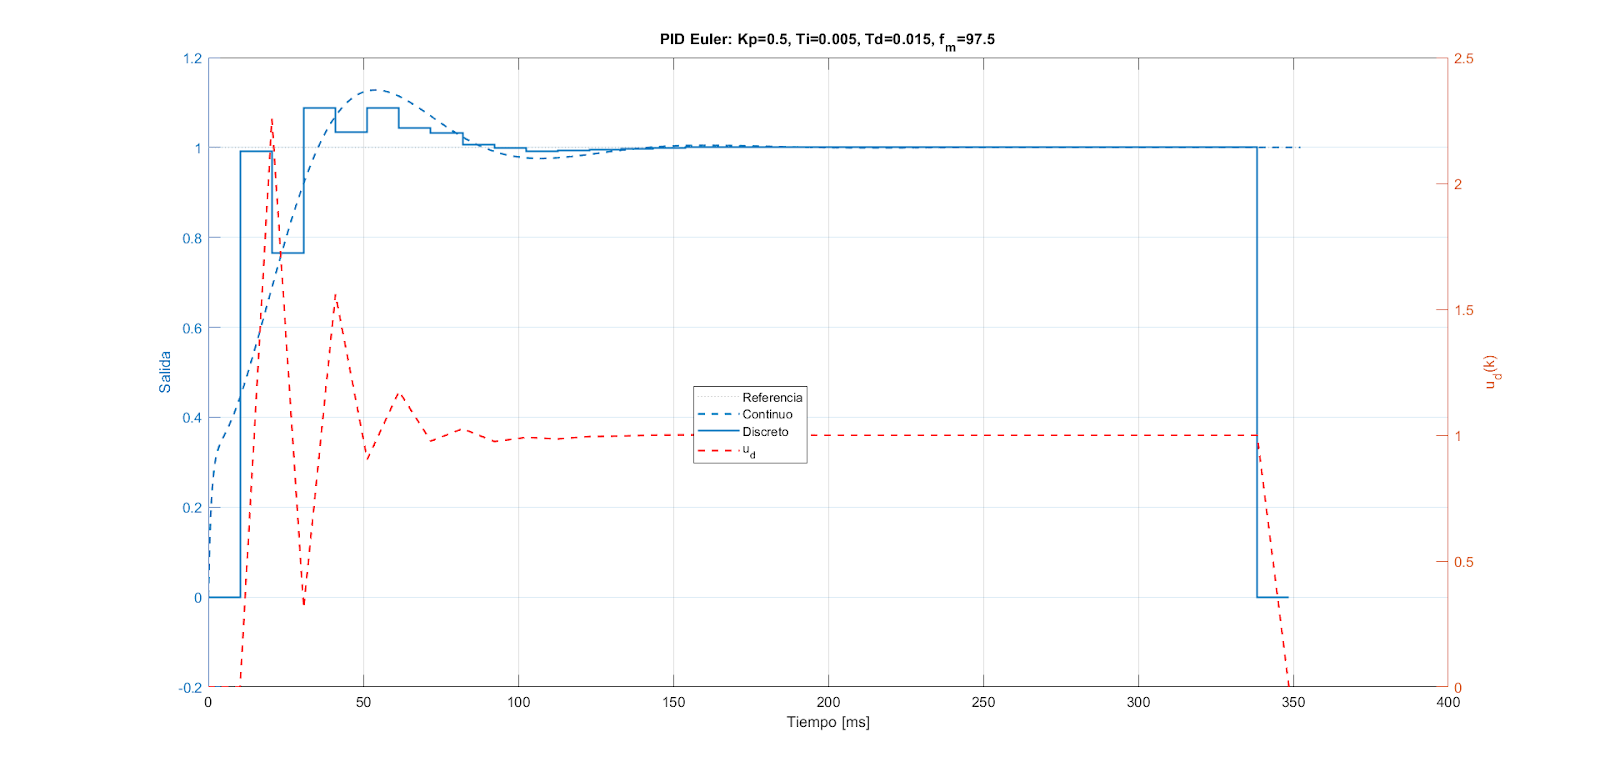
\includegraphics[width=\columnwidth]{img/fs10.png}
	\caption{Respuesta con $f_s=10 f_{\mathrm{bw}}$: la discretización no es suficiente y la respuesta discreta se aparta del continuo.}
	\label{fig:fs10}
\end{figure}



\subsubsection{ Implementación con un tiempo de muestreo de 30 veces el ancho de banda del sistema
}

Al triplicar la frecuencia de muestreo:
\[
f_s = 30 f_{\mathrm{bw}}, \qquad T = \frac{1}{f_s},
\]
Podemos ver en la Figura~\ref{fig:fs30} muestra una mejora clara: la respuesta discreta se asemeja mucho más a la continua, con menor error con respecto a la continua.

\begin{figure}[!t]
	\centering
	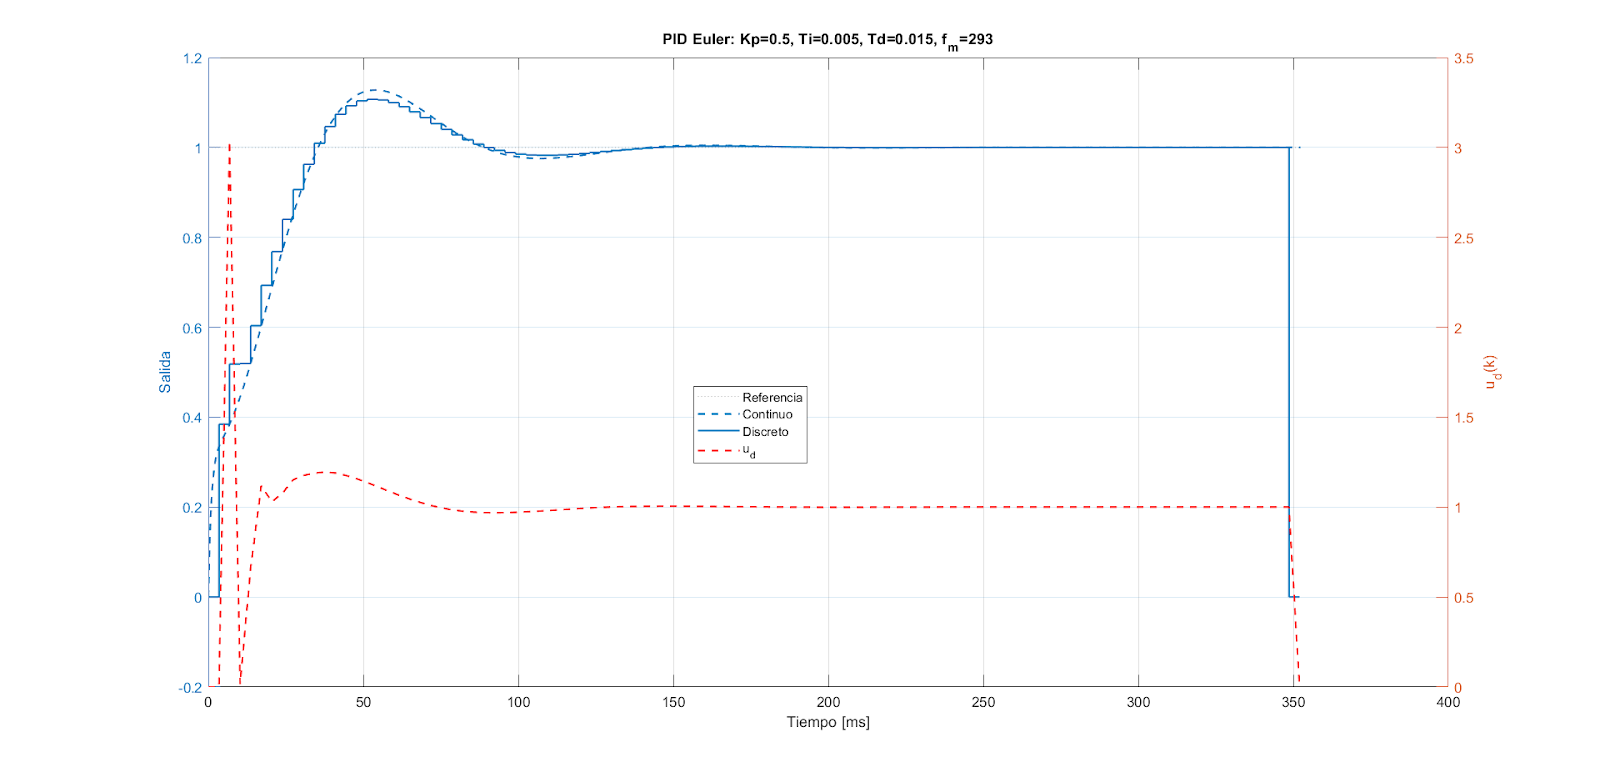
\includegraphics[width=\columnwidth]{img/fs30.png}
	\caption{Respuesta con $f_s=30 f_{\mathrm{bw}}$: el lazo discreto reproduce con mayor fidelidad al continuo.}
	\label{fig:fs30}
\end{figure}

\paragraph{Limitación con Ziegler--Nichols.}  
Al usar parámetros obtenidos con ZN, el control logra buen seguimiento, pero el esfuerzo de control $u_d[k]$ supera en más de dos órdenes de magnitud la capacidad de los DAC del PSoC (Figura~\ref{fig:zn_effort}). Esto vuelve la solución impracticable.

\begin{figure}[!t]
	\centering
	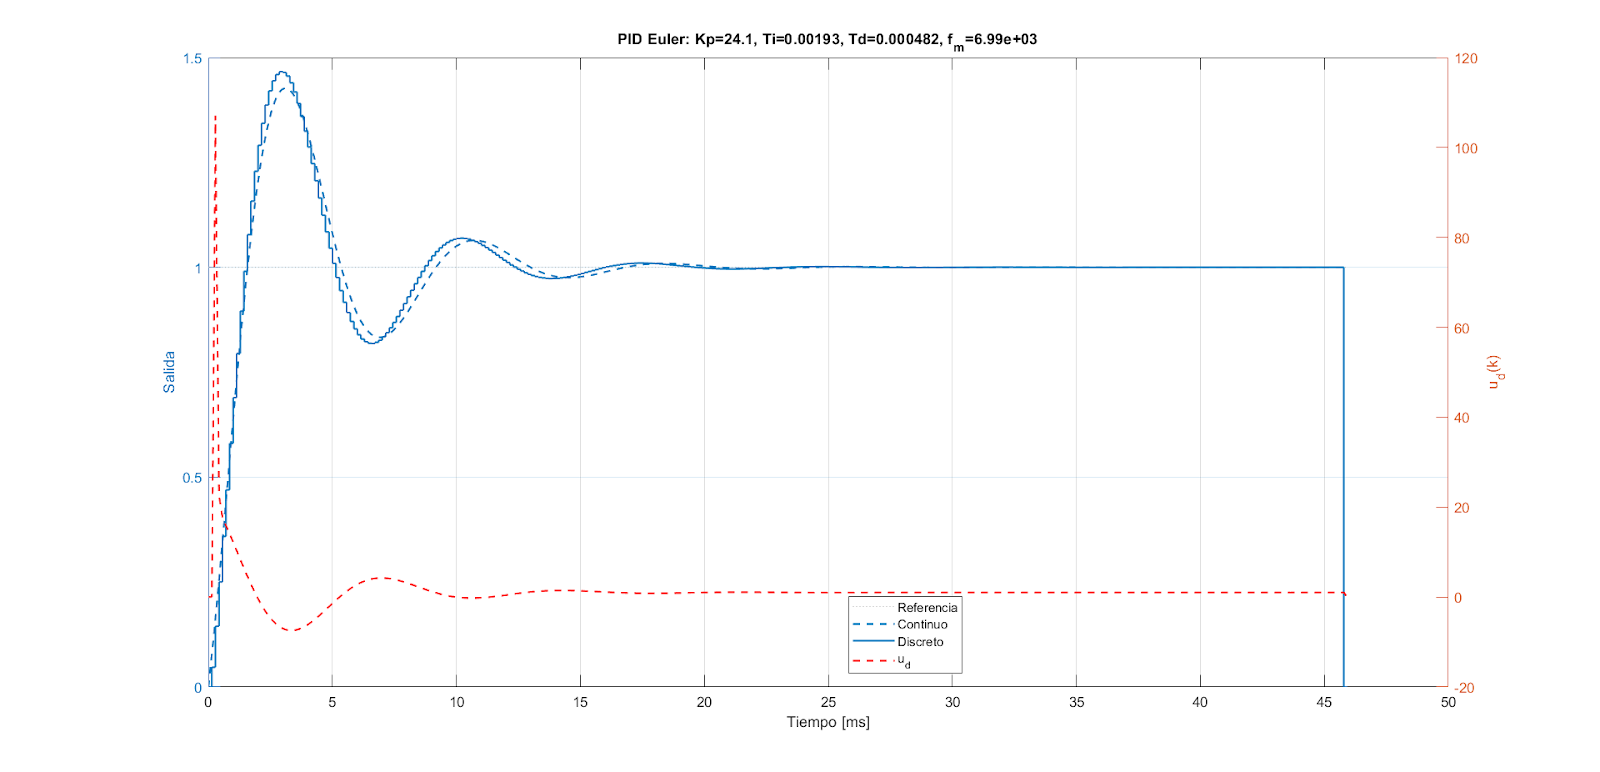
\includegraphics[width=\columnwidth]{img/zn_effort.png}
	\caption{Sintonía ZN: buena respuesta, pero esfuerzo $u_d[k]$ excesivo (no implementable).}
	\label{fig:zn_effort}
\end{figure}

Para evidenciarlo, añadimos ruido y saturación al esfuerzo en la simulación. El resultado (Figura~\ref{fig:sat_noise}) confirma que el sistema no puede seguir al escalón bajo esas condiciones.

\begin{figure}[!t]
	\centering
	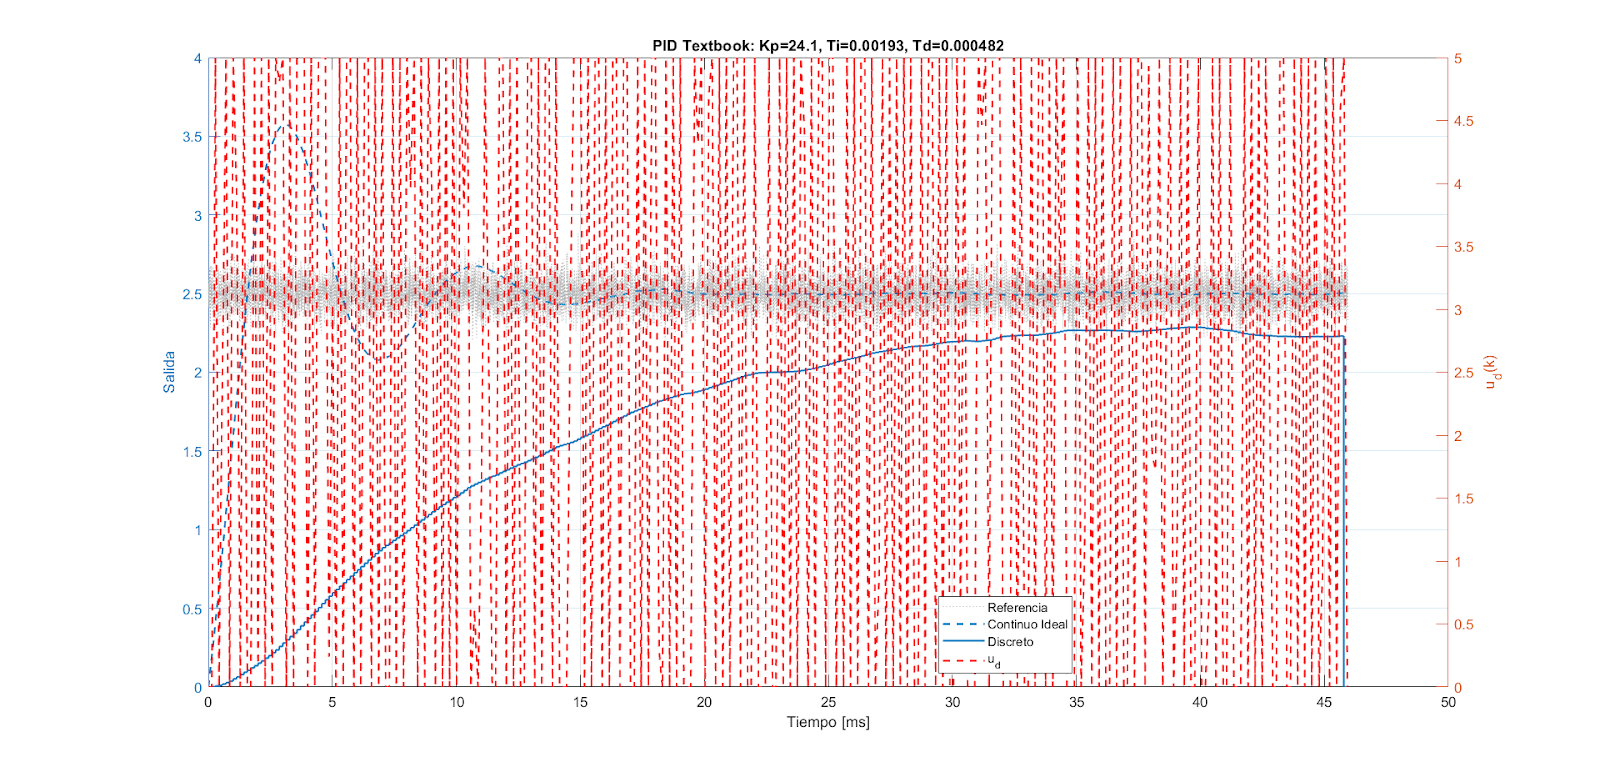
\includegraphics[width=\columnwidth]{img/sat_noise.png}
	\caption{PID discreto con ruido y saturación: se observa windup y pérdida total del seguimiento.}
	\label{fig:sat_noise}
\end{figure}


\onecolumn
\subsubsection*{Simulación con saturación y ruido}

La función utilizada en la sección anterior es la siguiente:

\begin{lstlisting}[language=Matlab,style=matlabstyle, caption={PID discreto con saturación y ruido}, label={lst:pid_sat_noise}]
	function sim_pid_euler(G, T, Kp, Ti, Td, stepSize, sigma, umin, umax)
	% --- Control continuo (referencia) ---
	numC = Kp*[Ti*Td, Ti, 1]; denC = [Ti, 0];
	controlador = tf(numC, denC);
	cloop_c = feedback(controlador*G, 1);
	info  = stepinfo(cloop_c);
	tend  = 3*info.SettlingTime;
	wn    = 1.8/info.RiseTime;
	Tstep = (2*pi/wn)/1000;
	t  = 0:Tstep:tend;
	td = 0:T:tend;
	
	% Referencia con ruido
	refc = stepSize*ones(size(t)) + sigma*randn(size(t));
	yc   = lsim(cloop_c, refc, t);
	refd = interp1(t, refc, td, 'linear', 'extrap');
	
	% --- Planta discreta (ZOH) ---
	Gd = c2d(G, T, 'zoh');
	[numD, denD] = tfdata(Gd, 'v');
	b0 = numD(2); b1 = numD(3);
	a1 = denD(2); a2 = denD(3);
	
	% Inicialización
	yd = zeros(size(td));
	ed = zeros(size(td));
	ud = zeros(size(td));
	
	% --- PID incremental con saturación ---
	for k = 3:numel(td)-1
	ed(k) = refd(k) - yd(k);
	u_inc = ud(k-1) + Kp*((1+T/Ti+Td/T)*ed(k) ...
	-(1+2*Td/T)*ed(k-1) ...
	+(Td/T)*ed(k-2));
	% Saturación
	if u_inc > umax
	ud(k) = umax;
	elseif u_inc < umin
	ud(k) = umin;
	else
	ud(k) = u_inc;
	end
	% Planta discreta
	yd(k+1) = b0*ud(k) + b1*ud(k-1) - a1*yd(k) - a2*yd(k-1);
	end
	
	% --- Gráficos ---
	yshift = circshift(yd, -2);
	figure; hold on; grid on;
	yyaxis left
	plot(t*1000, refc, ':','Color',[0.7 0.7 0.7]);
	plot(t*1000, yc,  '--','LineWidth',1.3);
	stairs(td*1000, yshift,'-','LineWidth',1.2);
	ylabel('Salida');
	yyaxis right
	plot(td*1000, ud, 'r--','LineWidth',1.2);
	ylabel('u_d[k]');
	xlabel('Tiempo [ms]');
	title(sprintf('PID discreto: Kp=%.3g, Ti=%.3g, Td=%.3g', Kp, Ti, Td));
	legend('Referencia','Continuo ideal','Discreto sat+ruido','u_d');
	end
\end{lstlisting}

\twocolumn

\subsubsection{Implementación del modelo alternativo y análisis con ruido y saturación}

Dado que la sintonía inicial de Ziegler--Nichols exige un esfuerzo de control incompatible con el actuador disponible, nos centramos en implementar el \emph{modelo alternativo} (PID ajustado por prueba y error con discretización incremental).  

\paragraph{Efectos del ruido (escenario amplificado).}
Para visualizar con claridad la sensibilidad al ruido (especialmente por el término derivativo), forzamos un caso más severo: desviación estándar del \(10\%\) de la amplitud de referencia. En la simulación:


\begin{lstlisting}[language=Matlab,breaklines=true,basicstyle=\ttfamily\footnotesize]
	sim_pid_euler(G,T/30,Kp,Ti,Td,2.5,0.25,0,5);
\end{lstlisting}

La Figura~\ref{fig:ruido_10pct} evidencia el efecto del ruido sobre \(u_d[k]\) y la salida discreta, pero sigue dando un resultado aceptable en el seguimiendo de la referencia aun en este caso extremo.

\begin{figure}[!t]
	\centering
	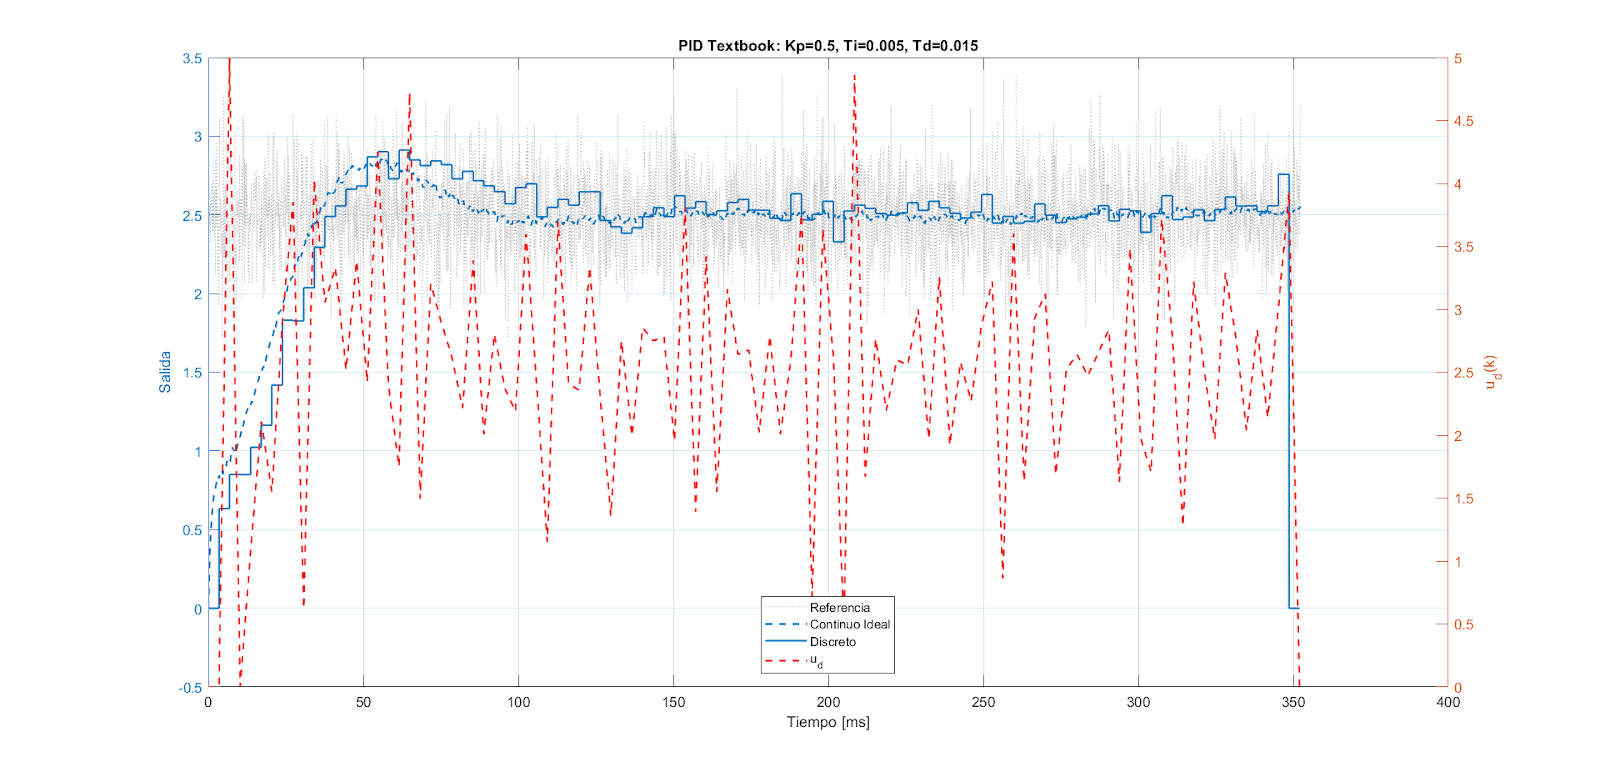
\includegraphics[width=\columnwidth]{img/ruido_10pct.png}% <-- exportá esta imagen
	\caption{Caso ruidoso (sigma $=10\%$ de la amplitud): ondulación amplificada por sensibilidad del término derivativo.}
	\label{fig:ruido_10pct}
\end{figure}

\paragraph{Efectos de la saturación (windup) sin ruido.}
Para aislar el fenómeno de \emph{windup} quitamos el ruido y exigimos amplitud elevada, manteniendo límites del actuador:
\begin{lstlisting}[language=Matlab,breaklines=true,basicstyle=\ttfamily\footnotesize]
	sim_pid_euler(G,T/30,Kp,Ti,Td,5,0,0,5);
\end{lstlisting}

La Figura~\ref{fig:windup} muestra la saturación de \(u_d[k]\) y la consecuente degradación del seguimiento: lento despegue y respuesta sobreamortiguada.

\begin{figure}[!t]
	\centering
	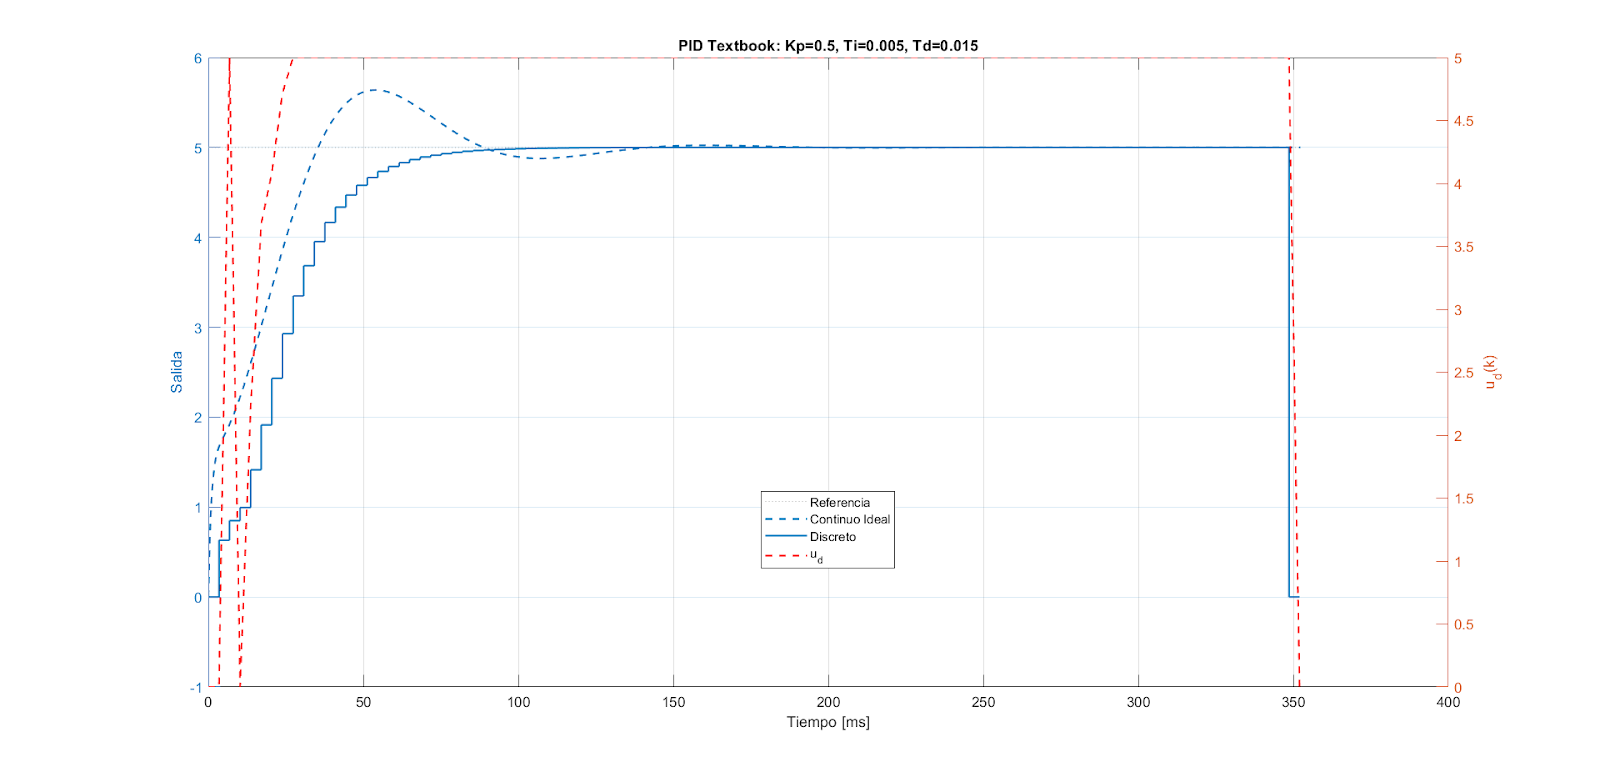
\includegraphics[width=\columnwidth]{img/windup.png}% <-- exportá esta imagen
	\caption{Caso con saturación y sin ruido: evidencia de windup e imposibilidad de seguimiento para amplitudes elevadas.}
	\label{fig:windup}
\end{figure}
